\documentclass[xcolor={dvipsnames}]{beamer}
%\usepackage[margin=1.0in]{geometry}

\usepackage[utf8]{inputenc}
\usepackage[english]{babel}
\usepackage[T1]{fontenc}
\usepackage{lmodern}

%----------------------------------------------------------------------------------------
%	MATH PACKAGES
%----------------------------------------------------------------------------------------

% Banish \phi from this realm
\renewcommand{\phi}{\varphi}

\usepackage{amsmath, amssymb, mathrsfs}
\usepackage{mathtools}

%----------------------------------------------------------------------------------------
%	DEFINING NEW FUNCTIONS
%----------------------------------------------------------------------------------------

% --------- MATH MODE ---------
% Equation numbering per section
\numberwithin{equation}{section}

% \cdot instead of asterisk (*) symbol
\mathcode`\*="8000
{\catcode`\*\active\gdef*{\cdot}}

% --------- OTHER ---------

\usepackage[dvipsnames]{xcolor}

% tikz
%\usepackage{tikz}

% Captions
\usepackage[font=scriptsize]{caption}

% Quotes
\usepackage[autostyle=false]{csquotes}
\newcommand{\q}[1]{„#1''} % Redefine quotations

\usetheme{Madrid}
\usecolortheme{default}
\setbeamertemplate{caption}[numbered]

\newif\ifplacelogo
\placelogotrue
%----------------------------------------------------------------------------------------
%	TITLE PAGE
%----------------------------------------------------------------------------------------
\title[Geant4]
{Simulation of the NEBULA detector using Geant4}

\subtitle{Midterm presentation}

\author[Balázs Pál]
{Balázs Pál}

\institute[ELTE]
{
  Supervisor : Ákos Horváth, PhD \newline
  Eötvös Loránd University
}

\date[ELTE 2021]
{Scientific Modelling Computer Lab, March 24, 2021}

\logo{\ifplacelogo
\includegraphics[height=1.5cm]{./images/elte-logo.jpg}\fi}

\begin{document}

\frame{\titlepage}
%----------------------------------------------------------------------------------------
%	SLIDE 1.
%----------------------------------------------------------------------------------------
\begin{frame}
\frametitle{Simulation of the NEBULA detector}

\begin{block}{Initial considerations}
	\begin{itemize}
		\item Installing smsimulator, which uses libraries from ROOT and ANAROOT and headers and binaries from Geant4
		\item This software could be used to simulate the NEBULA detector with very high accuracy
		\item Installing and configuring it seems to be a nightmare currently
	\end{itemize}
\end{block}

\pause

\begin{alertblock}{Changed roadmap}
	\begin{itemize}
		\item Temporarily abort the idea of using smsimulator
		\item Implementing a simplified version of the NEBULA  detector
		\item It should be still able to give good approximations
	\end{itemize}
\end{alertblock}

\end{frame}
%----------------------------------------------------------------------------------------
%	SLIDE 2./1
%----------------------------------------------------------------------------------------
\begin{frame}
\frametitle{Making NEBULA rods susceptible for neutrons}

\begin{exampleblock}{Structure of the simulated detector}
	\begin{itemize}
		\item $2 \times 10$ plastic scintillator rods in two layers
		\item Dimensions of rods are $12\text{cm} \times 12\text{cm} \times 180\text{cm}$
	\end{itemize}
\end{exampleblock}

\begin{figure}
	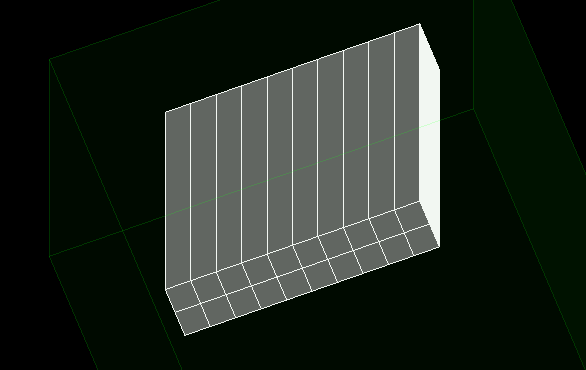
\includegraphics[width=0.5\textwidth]{images/nebula.png}
\end{figure}


\end{frame}
%----------------------------------------------------------------------------------------
%	SLIDE 2./2
%----------------------------------------------------------------------------------------
\begin{frame}
\frametitle{Making NEBULA rods susceptible for neutrons}

\begin{block}{\texttt{G4SteppingAction}}
	\begin{itemize}
		\item Handles the individual tracking of each particle in the simulation
	\end{itemize}
\end{block}

\begin{block}{\texttt{G4LogicalVolume} : Initialized in \texttt{G4DetectorConstruction}}
	\begin{itemize}
		\item Geant4's \texttt{G4SteppingAction} can use this type of volume to identify the mother volume of the particle's position in the current step
		\item This type of volume contains the methods used for particle tracking
	\end{itemize}
\end{block}

\begin{alertblock}{\texttt{G4Accumulable} : Initialized in \texttt{G4RunAction}}
	\begin{itemize}
		\item Stores "accumulable" quantities (eg. energies) during the whole simulation
		\item The \texttt{G4AnalysisManager} reads values from this type of object
	\end{itemize}
\end{alertblock}


\end{frame}
%----------------------------------------------------------------------------------------
%	SLIDE 3.
%----------------------------------------------------------------------------------------
\begin{frame}
\frametitle{Simulations in Geant4}
\framesubtitle{Very short outline}

\begin{block}{Usual components}
	\begin{itemize}
		\item Detector construction
		\item Particle generation
		\item Data I/O
		\item Core loop
	\end{itemize}
\end{block}

\end{frame}
%----------------------------------------------------------------------------------------
%	SLIDE 4./1.
%----------------------------------------------------------------------------------------
\begin{frame}
\frametitle{Analysis of simulation results}

\begin{exampleblock}{}
	\begin{itemize}
		\item All neutrons are set to have the same amount of energy at the start (tested for $20$, $100$, $200$ and $300$ MeVs)
		\item The NEBULA rods measure the deposited energies for each particles penetrating them
	\end{itemize}
\end{exampleblock}

\begin{figure}
	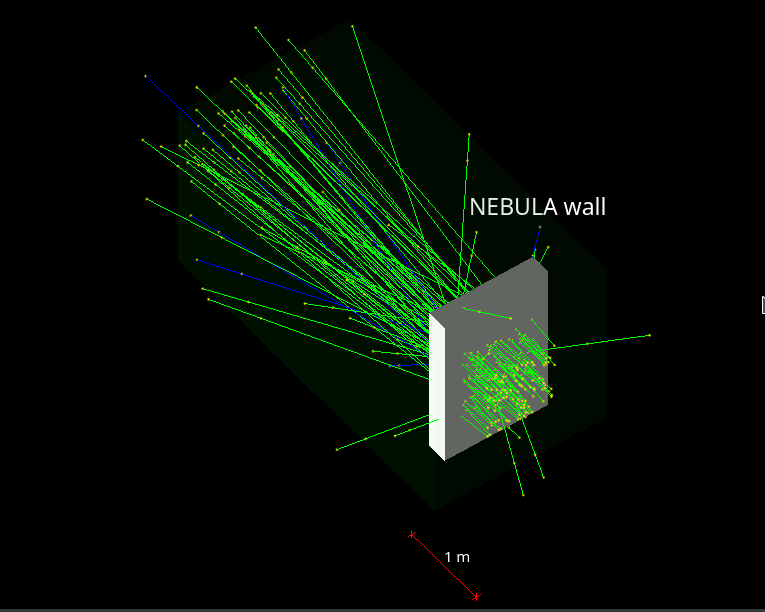
\includegraphics[width=0.5\textwidth]{images/nebula_3d.png}
\end{figure}

\end{frame}
\placelogofalse
%----------------------------------------------------------------------------------------
%	SLIDE 4./2.
%----------------------------------------------------------------------------------------
\begin{frame}
\frametitle{Analysis of simulation results}

\begin{figure}
	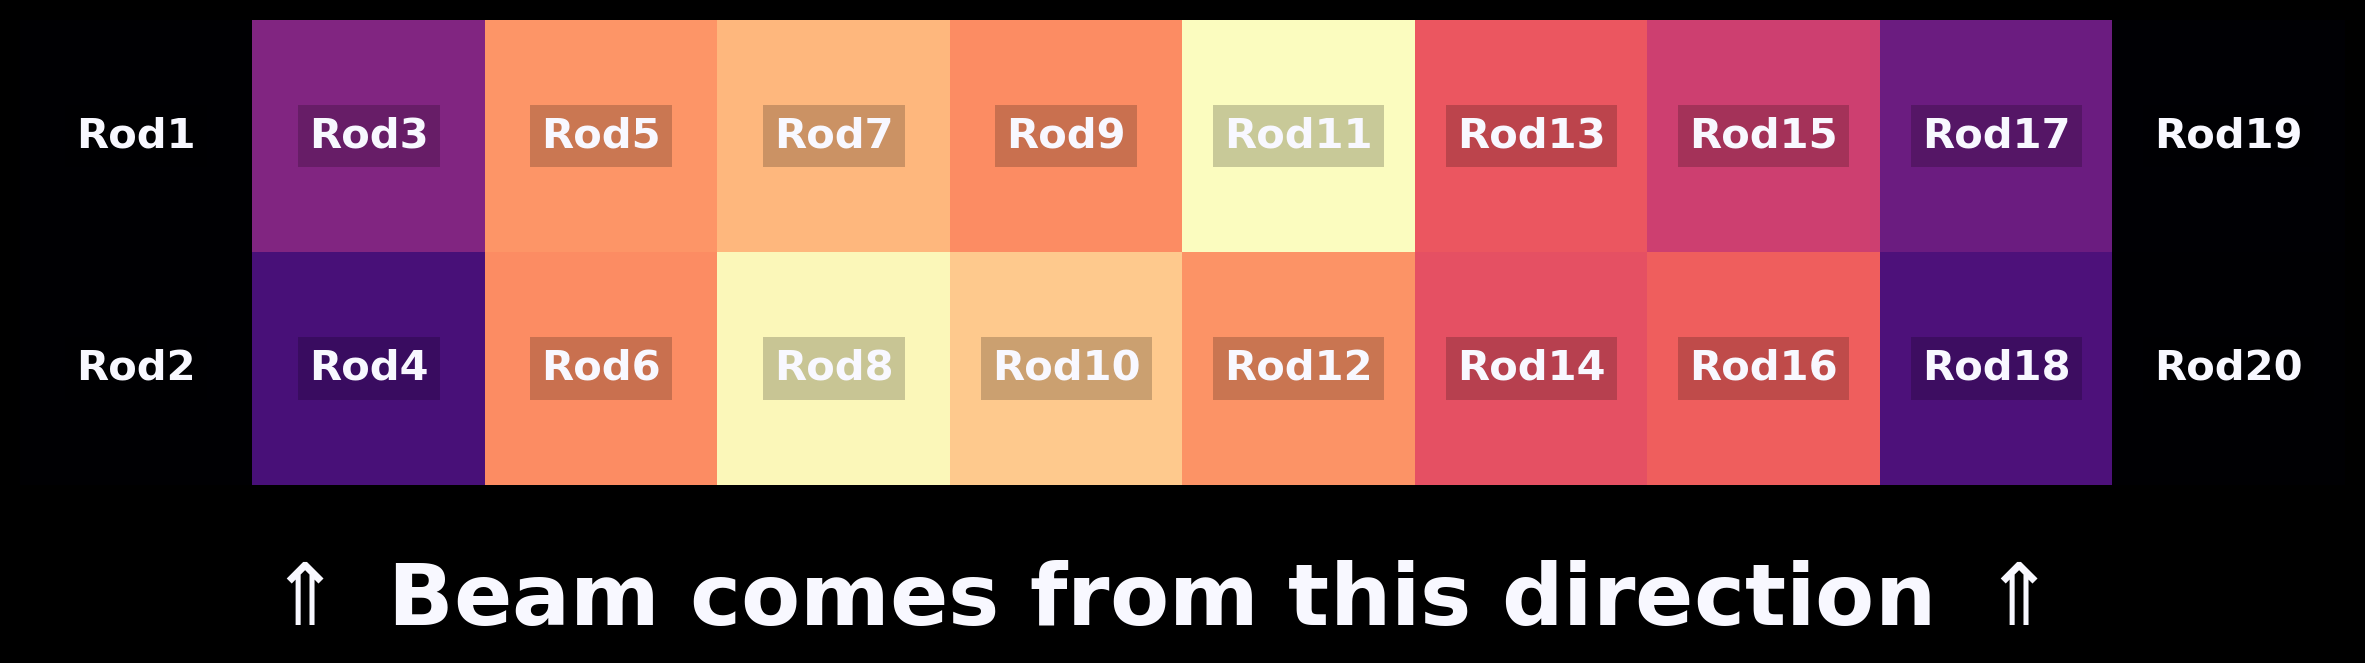
\includegraphics[width=0.86\textwidth]{images/rod_heatmap_100.png}
	\captionof{figure}{Heatmap of the total deposited energy in the NEBULA detector rods during a test run of $1000$ neutrons of $100$ MeV.}
\end{figure}

\begin{figure}
	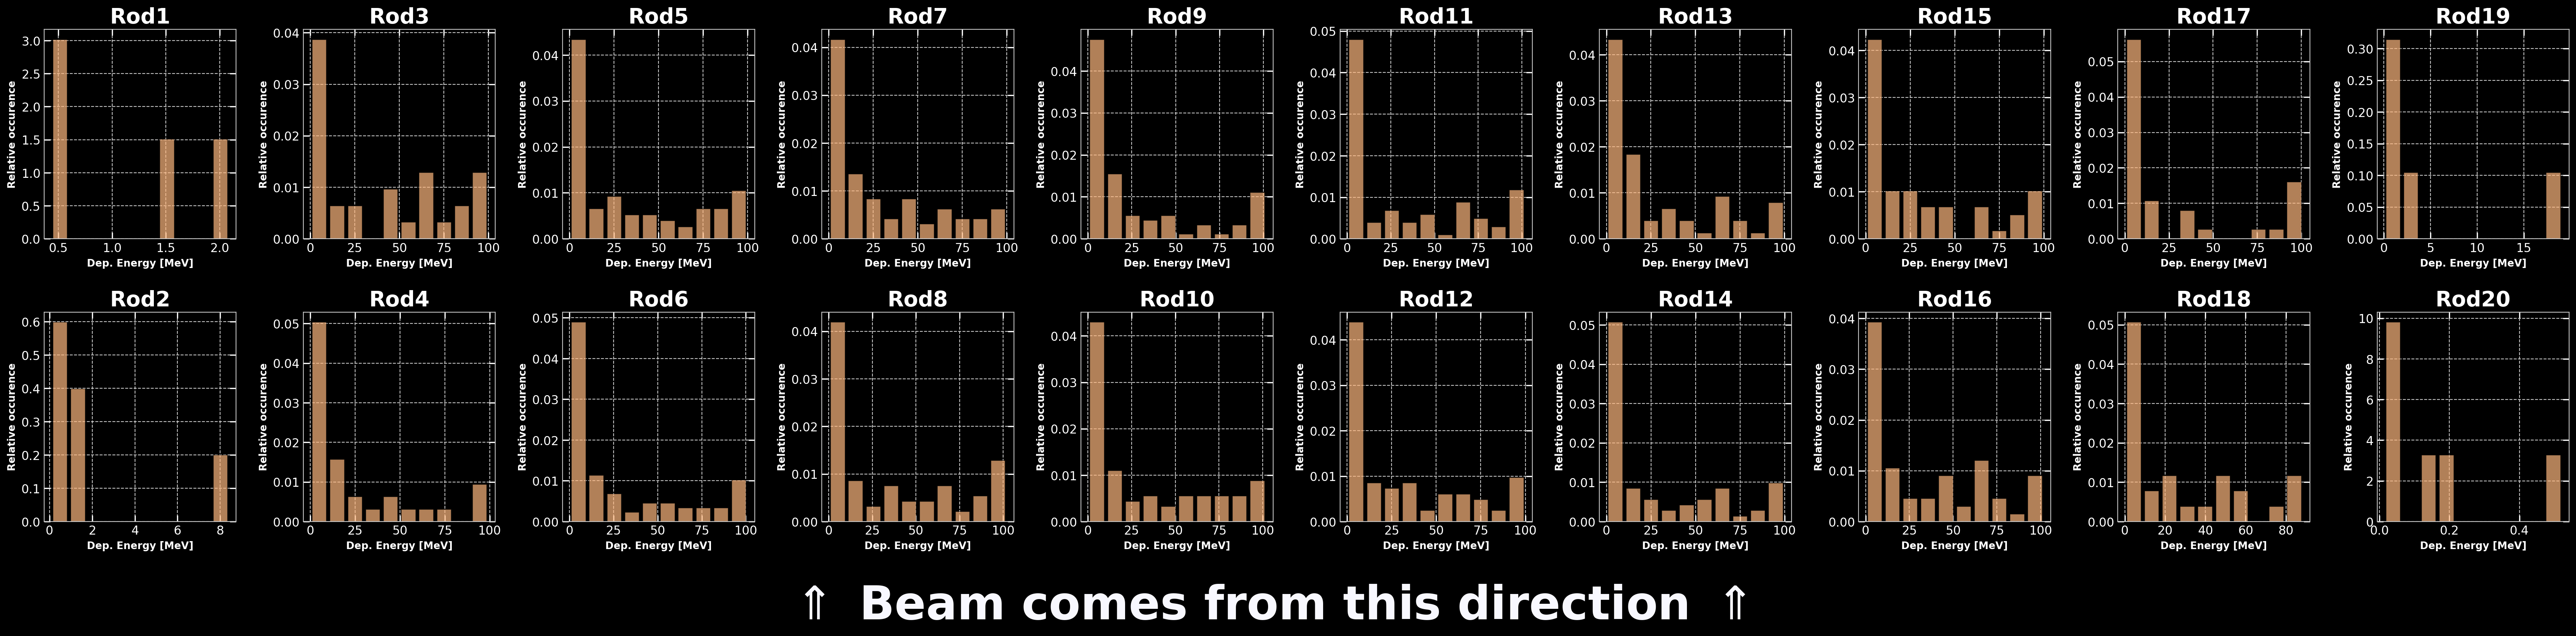
\includegraphics[width=0.86\textwidth]{images/energy_dist_per_rod_100.png}
	\captionof{figure}{Histogram of the deposited energies for each NEBULA detector rods during a test run of $1000$ neutrons of $100$ MeV.}
\end{figure}

\end{frame}
\placelogotrue


\end{document}